Gegeben ist die Funktion
\begin{equation}
\varphi(x)
=
\begin{cases}
a(\cosh 1 - \cosh x)&\qquad -1\le x \le 1
\\
0&\qquad\text{sonst,}
\end{cases}
\label{50000040:varphi}
\end{equation}
wobei die hyperbolische Kosinus-Funktion definiert ist durch
\[
\cosh x = \frac{e^x + e^{-x}}{2}.
\]

\begin{figure}[h]
\centering
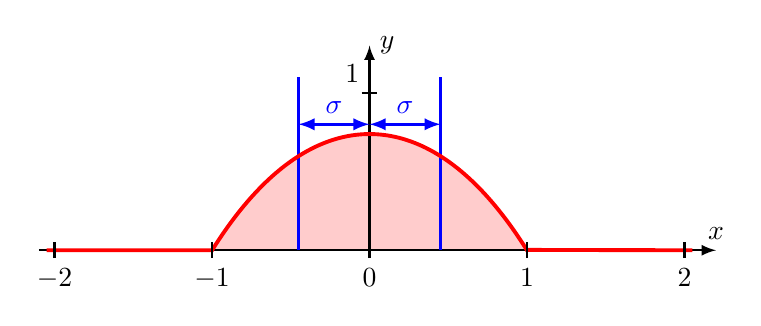
\begin{tikzpicture}[>=latex,thick,scale=2]
\def\a{1.359141}
\fill[color=red!20]
	plot[domain=-1:1,samples=100] ({\x},{\a*(exp(1)+exp(-1)-exp(\x)-exp(-\x))/2})--cycle;
\draw[->] (-2.1,0)--(2.2,0) coordinate[label={$x$}];
\draw[->] (0,-0.05)--(0,1.3) coordinate[label={right:$y$}];
\ifthenelse{\boolean{loesungen}}{
\draw[color=blue,line width=1pt] (0.451274,0)--(0.451274,1.1);
\draw[color=blue,line width=1pt] (-0.451274,0)--(-0.451274,1.1);
\draw[<->,line width=1pt,color=blue] (-0.451274,0.8)--(0,0.8);
\draw[<->,line width=1pt,color=blue] (0.451274,0.8)--(0,0.8);
\node[color=blue] at (-0.225,0.8) [above] {$\sigma$};
\node[color=blue] at (0.225,0.8) [above] {$\sigma$};
}{}
\draw[color=red,line width=1.4pt]
	(-2.05,0)--(-1,0)
	--
	plot[domain=-1:1,samples=100] ({\x},{\a*(exp(1)+exp(-1)-exp(\x)-exp(-\x))/2})
	--
	(2.05,0);
\draw (-2,-0.05)--(-2,0.05);
\draw (-1,-0.05)--(-1,0.05);
\draw ( 1,-0.05)--( 1,0.05);
\draw ( 2,-0.05)--( 2,0.05);
\draw (-0.05,1)--(0.05,1);
\node at (-2,-0.05) [below] {$-2$};
\node at (-1,-0.05) [below] {$-1$};
\node at (0,-0.05) [below] {$0$};
\node at (1,-0.05) [below] {$1$};
\node at (2,-0.05) [below] {$2$};
\node at (0,1) [above left] {$1$};
\end{tikzpicture}
\caption{Funktion $\varphi(x)$ \eqref{50000040:varphi} für
Aufgabe~\ref{50000040}
\label{50000040:graph}}
\end{figure}
\begin{teilaufgaben}
\item
Für welche Werte des Parameters $a$ ist die $\varphi(x)$
eine Wahrscheinlichkeitsdichte?
\item
Bestimmen Sie den Erwartungswert einer Zufallsvariablen mit dieser 
Verteilung.
\item
Bestimmen Sie die Varianz einer Zufallsvariablen mit dieser
Verteilung.
\end{teilaufgaben}

\begin{hinweis}
Für die manuelle Berechnung können Sie die Formeln
\[
\sinh x = \frac{e^x - e^{-x}}2,\qquad
\frac{d}{dx}\cosh x = \sinh x, \qquad
\frac{d}{dx}\sinh x = \cosh x
\]
verwenden.
\end{hinweis}

\begin{loesung}
\begin{teilaufgaben}
\item
Die Normierungsbedingung
\[
\int_{-\infty}^\infty \varphi(x)\,dx =1
\]
muss erfüllt sein.
Wir berechnen
\begin{align*}
1
&=
a\int_{-1}^1 \cosh 1 - \cosh x\,dx
=
a\biggl[ x \cosh 1 - \sinh x\biggr]_{-1}^1
=
a(2\cosh1 -2\sinh 1)
\\
&=
a(e + e^{-1} - e + e^{-1})
=
2ae^{-1}
\\
\Rightarrow\quad
a&=\frac{e}{2}=1.359141.
\end{align*}
\item
Da $\varphi$ eine gerade Funktion ist, ist $E(X)=0$.
\item
Es muss nur noch $E(X^2)$ berechnet werden.
Es gilt
\begin{align*}
E(X^2)
&=
\int_{-\infty}^\infty x^2\varphi(x)\,dx
=
a\int_{-1}^1 x^2 (\cosh 1 - \cosh x)\,dx
\\
&=
a\cosh 1\cdot \biggl[\frac{x^2}{3}\biggr]_{-1}^1
-
a\biggl[\sinh x\biggr]_{-1}^{1}
+
2a\int_{-1}^1 x\sinh x\,dx
\\
&=
\frac{2a}{3}\cosh 1 - 2a\sinh 1
+2a\biggl[x\cosh x\biggr]_{-1}^1
-2a\int_{-1}^1 \cosh x\,dx
\\
&=
\frac{2a}{3}\cosh 1
 - 2a\sinh 1
+2a\cosh 1
-2a\biggl[\sinh x\biggr]_{-1}^1
\\
&=
\frac{2a}{3}\cosh 1
 - 2a\sinh 1
+4a\cosh 1
-4a\sinh 1
\\
&=
\frac{e}{3}
(\cosh 1 -3\sinh 1 + 6\cosh 6 - 6\sinh 1)
=
\frac{e}{3}(7\cosh 1 - 9 \sinh 1)
\\
&=
\frac{e}{3}(-e+8e^{-1})
=
\frac{8-e^2}{3}
=
0.203648
\\
\Rightarrow\qquad
\sqrt{\operatorname{var}(X)}
=
\sigma
&=
0.451274.
\end{align*}
$\sigma$ ist ebenfalls in der Abbildung~\ref{50000040:graph} eingezeichnet.
\qedhere
\end{teilaufgaben}
\end{loesung}

\begin{bewertung}
\begin{teilaufgaben}
\item
Normierungsbedingung ({\bf N}) 1 Punkt,
Wert von $a$ ({\bf A}) 1 Punkt.
\item
Formel für Erwartungswert $E(X)=\int x\varphi(x)\,dx$
oder Berechnung mit Symmetrie ({\bf E}) 1 Punkt.
\item
Formel für Erwartungswert $E(X^2)$  ({\bf X$\mathstrut^2$}) 1 Punkt,
Formel für Varianz $\operatorname{var}(X) = E(X^2)-E(X)^2$ ({\bf V}) 1 Punkt,
Zahlenwert für die Varianz ({\bf Z}) 1 Punkt.
\end{teilaufgaben}
\end{bewertung}

